% D-, E- and A-optimal gene panels for vignette 03-1, #fig-dea-design.
% Panels: scripts/figures/fig_03_1_dea_design.R (ggplot2); numbers: ledger V18.
% Build: latexmk -lualatex dea_design.tex; pdftocairo -svg dea_design.pdf
%        ../../fig_03_1_dea_design.svg
\documentclass[tikz,border=4pt]{standalone}
\usepackage{iftex}
\ifPDFTeX
  \PackageError{dea_design}{Use LuaLaTeX or XeLaTeX}{}
\fi
\usepackage{fontspec}
\usepackage{amsmath,amssymb,amsfonts,bm}
\usepackage{graphicx}
\usetikzlibrary{arrows.meta,positioning,fit,backgrounds,calc,shapes.geometric}
% palette and flowchart styles of vignettes/_quarto.yml
\definecolor{ink}{HTML}{1F2937}
\definecolor{latfill}{HTML}{DAE9FB}
\definecolor{latdraw}{HTML}{4477B5}
\definecolor{obsfill}{HTML}{C9CDD3}
\definecolor{obsdraw}{HTML}{747B86}
\tikzset{
  every node/.style={text=ink},
  edge/.style={-{Stealth[length=2.6mm]}, line width=0.8pt, draw=ink},
  box/.style={rectangle, rounded corners=3pt, draw=ink, fill=white, line width=0.8pt,
    align=center, inner sep=1.6mm, font=\small},
  keybox/.style={box, draw=latdraw, fill=latfill},
  dimbox/.style={box, draw=obsdraw, fill=obsfill!45},
  panel/.style={inner sep=0pt, anchor=north west},
  tag/.style={font=\bfseries\small, anchor=north west, inner sep=1pt}
}
\begin{document}
\begin{tikzpicture}
  \node[panel] (A) at (0,0) {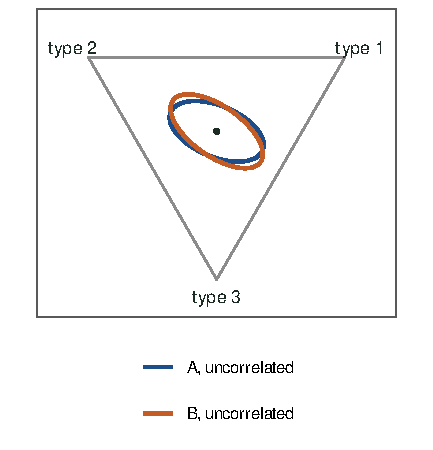
\includegraphics[width=6.6cm]{panel_a_independent.pdf}};
  \node[panel] (B) at (7.0,0) {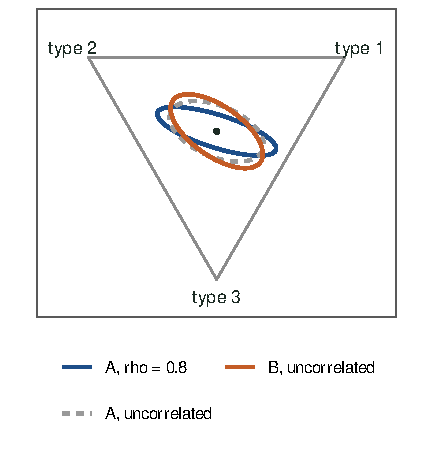
\includegraphics[width=6.6cm]{panel_b_correlated.pdf}};
  \node[panel] (C) at (14.0,0) {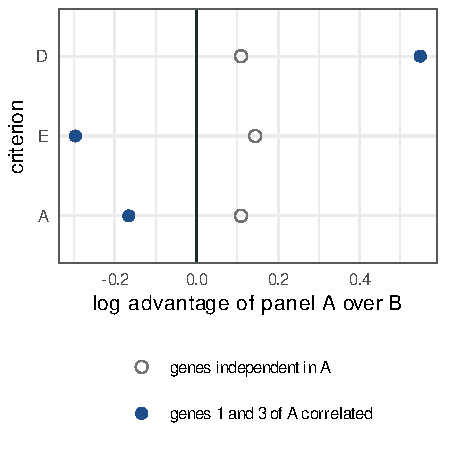
\includegraphics[width=6.8cm]{panel_c_criteria.pdf}};
  \node[tag] at (A.north west) {a};
  \node[tag] at (B.north west) {b};
  \node[tag] at (C.north west) {c};
  % shared information matrix
  \node[keybox, above=3mm of B, text width=19.5cm] (info)
    {$J=3$ types, two candidate panels of $G=3$ genes, common within-type covariance
    $\boldsymbol{\Sigma}_W$:\quad
    $\boldsymbol{I}=n_i\,\boldsymbol{K}^{\top}\boldsymbol{M}^{\top}\boldsymbol{\Sigma}_W^{-1}
    \boldsymbol{M}\boldsymbol{K}$,\quad
    $\operatorname{Cov}\hat{\boldsymbol{p}}=\boldsymbol{K}\boldsymbol{I}^{-1}\boldsymbol{K}^{\top}$
    ($\boldsymbol{K}$ orthonormal, columns orthogonal to $\mathbf{1}$); 95\,\% ellipses at
    $\boldsymbol{p}=(\tfrac13,\tfrac13,\tfrac13)$, $n_i=25$};
  % panel captions with the criteria
  \node[dimbox, below=2mm of A, text width=6.3cm] (cA)
    {$\boldsymbol{\Sigma}_W=\boldsymbol{I}$: $\boldsymbol{I}=n_i\boldsymbol{A}^{\top}\boldsymbol{A}$,
    $\boldsymbol{A}=\boldsymbol{M}\boldsymbol{K}$;\\
    $\det\boldsymbol{I}\propto$ squared Gram volume,
    $\kappa(\boldsymbol{I})=\kappa(\boldsymbol{A})^2$.\\
    Panel A wins on D, E and A};
  \node[dimbox, below=2mm of B, text width=6.3cm] (cB)
    {Correlation $0.8$ between genes 1 and 3 of panel A:\\
    smaller area (D prefers A),\\
    longer major axis (E and A prefer B)};
  \node[dimbox, below=2mm of C, text width=6.5cm] (cC)
    {D: $\max\det\boldsymbol{I}$ $\leftrightarrow$ ellipse area\\
    E: $\max\lambda_{\min}(\boldsymbol{I})$ $\leftrightarrow$ longest semi-axis\\
    A: $\min\operatorname{tr}\boldsymbol{I}^{-1}$ $\leftrightarrow$ sum of squared semi-axes};
  \draw[edge] ($(A.east)+(-0.2,0.6)$) -- node[above, font=\footnotesize] {$\rho_{13}$}
    ($(B.west)+(0.2,0.6)$);
\end{tikzpicture}
\end{document}
